%% This is an example first chapter.  You should put chapter/appendix that you
%% write into a separate file, and add a line \include{yourfilename} to
%% main.tex, where `yourfilename.tex' is the name of the chapter/appendix file.
%% You can process specific files by typing their names in at the 
%% \files=
%% prompt when you run the file main.tex through LaTeX.
\chapter{Implementation}\label{intro-ch}

\section{Spark}

All of the code was being implemented in Spark. As mentioned before, Spark is the next 
generation of map reduce and has received a huge amount of support. Although the code was implemented in Spark, 
it could also be implemented in map reduce to achieve similar gains. Matei Zaharia added code 
that allowed the tracking of sizes of map output files.   

\section{ShuffledRDD}

As mentioned before, the RDD is the main interface to interact with data in Spark.
The RDD we developed we developed basically is a new version of ShuffledRDD. Our version
of ShuffledRDD2 is basically a new version of the RDD. It takes in a shuffle dependency
, which is basically a bunch of partitions that have finished the map output stage. As mentioned before,
in a general ShuffledRDD just does basic logic, and does not do balancing. Our dependency
basically takes in a number of reducers and then best tries to balance the partitions of the reducer.
As this is more a proof of concept, our version of ShuffledRowRDD will only output consecutive partitions to one
reducer. In other words, it is impossible for a reducer to have partitions 1 and 3, without having partition 2. 
In the future, we hope to expand the RDD so that it best balances the parttions.

\section{Joins}

\subsection{ShuffleReader Changes}

We added some flexibility to how shuffles are fetched. As mentioned in the shuffle section,
we would like the bigger RDD to stay in place. The current interface allows a reducer to pick a specific partition
from the mapper and autofetched it from all of the mappers. In other words, you could only request partition 1 from
all the mappers. This would be extremely problematic for the broadcast join as we want none of the bigger RDD to move
at all.   

\subsection{ShuffleJoin and BroadcastJoin RDD}

The following example in Figure~\ref{fig:shuffle_basic} details the inner workings 
\begin{figure}[h]
\begin{center}
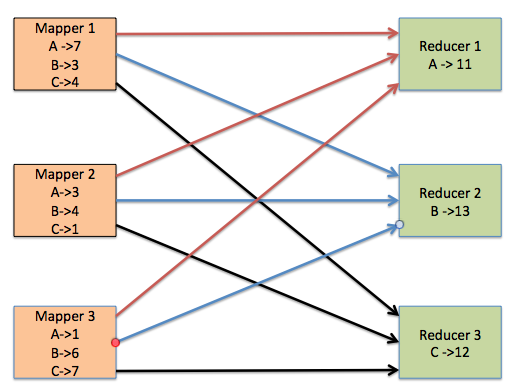
\includegraphics[scale=1.0]{./img/shuffle_basic.png}
\caption{Shuffle for Letter Count in Map Reduce}
\label{fig:shuffle_basic}
\end{center}
\end{figure}


